%------------------------------------------------------------------------------
% dxtbx: the diffraction experiment toolbox
%------------------------------------------------------------------------------

%\documentclass{iucr}
\documentclass[preprint]{iucr}

  %----------------------------------------------------------------------------
  % Extra packages
  %----------------------------------------------------------------------------
  \usepackage{graphicx}         % For graphics
  \usepackage{mathtools}        % Math stuff
  \usepackage{bm}               % Bold in maths
  \usepackage{listings}         % Code snippets
  \usepackage{bold-extra}       % Bold mono space for code snippets
  \usepackage{url}              % For URLs
  \usepackage{xspace}           % Spacing in macros

  %----------------------------------------------------------------------------
  % Information about the paper
  %----------------------------------------------------------------------------
  \paperprodcode{a000000}
  \paperref{xx9999}
  \papertype{FA}
  \paperlang{english}

  %----------------------------------------------------------------------------
  % Information about journal
  %----------------------------------------------------------------------------
  \journalcode{D}
  \journalyr{2013}
  %\journaliss{1}
  %\journalvol{56}
  %\journalfirstpage{000}
  %\journallastpage{000}
  \journalreceived{\relax}
  \journalaccepted{\relax}
  \journalonline{\relax}

  %----------------------------------------------------------------------------
  % Bits of formatting used throughout document
  %----------------------------------------------------------------------------
  \newcommand{\cctbx}{\emph{cctbx}\xspace}
  \newcommand{\dxtbx}{\emph{dxtbx}\xspace}
  \newcommand{\dials}{\emph{DIALS}\xspace}

  %----------------------------------------------------------------------------
  % Configure the listing environment
  %----------------------------------------------------------------------------
  \lstset{ %
    basicstyle=\scriptsize
  }
  
  
\begin{document}

  %----------------------------------------------------------------------------
  % Title of the paper + short title for header
  %----------------------------------------------------------------------------
  \title{\dxtbx: the diffraction experiment toolbox}
  \shorttitle{\dxtbx}

  %----------------------------------------------------------------------------
  % Authors
  %----------------------------------------------------------------------------
  \author[a]{James}{Parkhurst}
  \author[b]{Aaron}{Brewster}
  \author[a]{Luis}{Fuentes-Montero}
  \author[c]{David}{Waterman}
  \author[b]{Johan}{Hattne}
  \author[a]{Alun}{Ashton}
  \author[b]{Nathaniel}{Echols}
  \author[a]{Gwyndaf}{Evans}
  \author[b]{Nicholas}{Sauter}
  \cauthor[a]{Graeme}{Winter}{graeme.winter@diamond.ac.uk}

  %----------------------------------------------------------------------------
  % Affiliations
  %----------------------------------------------------------------------------
  \aff[a]{Diamond Light Source \country{UK}}
  \aff[b]{Lawrence Berkeley National Laboratory \country{USA}}
  \aff[c]{STFC Rutherford Appleton Laboratory \country{UK}}
  \shortauthor{Parkhurst \emph{et al.}}

  %----------------------------------------------------------------------------
  % Create the title
  %----------------------------------------------------------------------------
  \maketitle

%------------------------------------------------------------------------------
% Synopsis
%------------------------------------------------------------------------------
\begin{synopsis}
Supply a synopsis of the paper for inclusion in the Table of Contents.
FIXME (James). 2 Sentences
\end{synopsis}

%------------------------------------------------------------------------------
% Abstract
%------------------------------------------------------------------------------
\begin{abstract}
Supply a synopsis of the paper for inclusion in the Table of Contents. FIXME 
(James). Add some text. Single paragraph
\end{abstract}

%------------------------------------------------------------------------------
% Introduction
%------------------------------------------------------------------------------
\section{Introduction}

Effective processing of X-ray diffraction data from single crystal diffraction
experiments strongly depends on having an accurate model of the experimental
geometry, which in turn depends on having the ability to read, with no loss of
information, the wide variety of data formats used for X-ray diffraction
experiments. While many experiments for macromolecular crystallography employ a
simple geometry - the "rotation method" popularised by Arndt and Wonnacott
\cite{Arndt1977} in which the rotation axis lies approximately
perpendicular to direct beam, roughly coincident with one detector axis and 
"beam centre" somewhere in the middle of the detector \cite{Rossmann1979} - the 
general diffraction experiment may employ a much more complex geometry, allowing
for the rotation and translation of the detector and the sample. Reliably
representing this geometry from a range of different descriptions requires both
a single general "language" for the expression and the ability to import the 
contents of a variety of instruments. This is complicated by the possibility of 
storing the information in different ways: for example, storing the beam centre 
in pixels or mm, or the order of the "x" and "y" coordinates. While universal 
adoption of standards such as imgCIF \cite{Bernstein2005} for the 
recording of X-ray diffraction data would resolve these challenges very quickly, 
take up of the standard has been slow. 

The task of developing a tool to uniformly read diffraction image headers and
data has been addressed more than once. The CCP4 DiffractionImage library
\cite{Remacle2007} was developed to support the DNA and xia2 projects, as
it was realised early on that reliable access to a range of image headers was
vital. This was, however, limited by a lack of extensibility and by assumptions
made early in the design that the experimental geometry would correspond to the
simple layout described above. More recent efforts, such as FabIO 
\cite{Knudsen2013}, help to allow general access to the data but have a lesser 
emphasis on the metadata so critical for crystallographic data and its analysis. 
The diffraction experiment toolbox (\dxtbx) was developed initially to support 
the use of xia2 \cite{Winter2009}, as an improvement to using DiffractionImage, 
with the aim of allowing a completely general and user extensible approach to 
the reading and interpreting of image data and metadata. More recently this has 
been incorporated into the \cctbx \cite{Grosse-Kunstleve2002} to support
developments for XFEL data analysis \cite{Sauter2013} and the development of
new integration software \dials (Diffraction Integration for Advanced Light
Sources.) This recent effort has included support to a variety of new detector
types, access to the raw data (as well as metadata) in a uniform manner and
support for multi-image formats such as HDF5.

%------------------------------------------------------------------------------
% Method
%------------------------------------------------------------------------------
\section{Method of operation}

\subsection{Basic Principles}

To overcome the problems experienced by previous efforts to create a general 
framework for reading X-ray diffraction data, the \dxtbx was designed with the 
following principles in mind.

\begin{itemize}
  \item The library should be capable of reading image data and metadata from 
  a wide variety of file formats employing different descriptions of the 
  experiment.
  \item Image and metadata should be presented to the user via a single unified 
  interface using standard conventions to describe the experimental geometry.
  \item The library should be extensible by the user without the need to contact 
  the library's maintainers.
  \item The library's interface should provide abstraction from the details of 
  the experimental setup. Implementation specific information should not be 
  needed in order to write general algorithms.
\end{itemize}

In order to achieve these aims, the \dxtbx implements an extensible plug-in 
framework, where users can add their own modules to handle input from different 
file formats with different data representations. At the cost of writing a small 
amount of Python code, the user can extend the library to support any bespoke 
file format and transform the metadata therein to adhere to the standard imgCIF 
representation that is used within the \dxtbx experimental models. It also 
implements a simple high-level interface that enables access to data from the 
entire image set across multiple file representations within a single unified 
interface.

Following the methodology of the \cctbx, the library is a hybrid system written 
in C++ and Python \cite{Grosse-Kunstleve2002} \cite{Abrahams2003}. 
Python lends itself well to rapid development and writing clean portable code. 
It also has an extensive standard library. Various language features facilitate 
the easy implementation of generic code with interchangeable components. There 
is however an overhead with the use of Python, due to the interpreted nature of 
the language, so the experimental models were implemented in C++ to allow them 
to be used within optimised algorithms written in C++ without entailing this 
overhead. The boost.python language binding framework was used to export the 
C++ interface for use in Python.

\subsection{Data model}

The \dxtbx data model can be split into three distinct components: the 
experimental models, the back-end "format" plug-in system, and the high-level 
ImageSet/ImageSweep interface. The way that these components interact is 
demonstrated in Figure 1.

The experimental geometry can be accessed through four container classes: the 
beam, goniometer, detector and scan. Internally these classes store the 
description of the experiment in the standard imgCIF convention \cite{Bernstein2005}. 
Of these, the beam, goniometer and scan act primarily as storage for the 
description of the experiment; however, the detector model is necessarily more 
complex, providing methods to perform ray intersection and a pixel to millimetre 
mapping function that can be configured to handle complex effects, such as 
parallax correction and arbitrary pixel alignments, transparently through a 
simple generic interface. This allows general algorithms to be developed using 
the experimental models without reference to the specifics of the experimental 
setup and hardware used. 

The back-end handles reading the image and metadata itself through a collection 
of automatically discoverable plug-in classes derived from the Format base 
class. A Format class is responsible for determining if it "understands" the 
input data representation and populating the experimental models; a number of 
Format classes for known detectors and data representations are already provided 
and users can provide their own format to handle bespoke image formats and data 
representations, as will be demonstrated later in the manuscript. The high-level 
ImageSet/ImageSweep interface is then used to encapsulate all the metadata 
describing the experiment and provide convenient access to both image data and 
experimental models.

\subsection{High-level interface}

Access to the experimental models and image data is provided through a high-level 
"ImageSet/ImageSweep" interface. An image sweep represents a series of images 
that have a well defined geometric relationship between adjacent pixels in 3D, 
e.g. a series of images taken using the rotation method. Where this relationship 
does not exist, e.g. for XFEL data, but the images are nonetheless part of a 
single dataset, the "image set" interface is used. Both classes provide 
convenient access to image data through a python list-style interface, where 
images in the set can be iterated over and subsets can be selected and used. 
The ImageSweep class, additionally, provides methods to extract arbitrary sized 
3D volumes from the images sequence. The ImageSet and ImageSweep classes are 
instantiated by a factory function from the input data representation.  

Internally, the ImageSweep and ImageSet classes retain a reference to either a 
SingleFileReader or MultiFileReader class that handles the reading of a sequence 
of images from a single file, such as an HDF5 \cite{TheHDFGroup2010} file, or 
multiple files, such as a collection of image files, respectively. Both reader 
classes implement a single interface allowing the ImageSweep and ImageSet 
classes to interact with different data storage representations in a generic 
way. Support for subsets of images is implemented using the "flyweight" pattern 
\cite{Gamma1994}, whereby multiple subsets accessed through the light-weight 
high-level interface retain a reference to a single reader that performs the 
heavy lifting. This has the advantage of reducing memory consumption when 
addressing multiple subsets of images; image caching is performed within the 
reader class and so multiple subsets will share a single image cache. However, 
since the reader classes are not guaranteed to be re-entrant, concurrent file 
access across sub-sweeps is currently not possible, although this may be 
implemented with no change to the external interface.

Although, the ImageSweep and ImageSet classes provide facilities to cache images 
to improve performance of repeated reads of the same image, in the general case, 
it is not wise or possible to cache all the images in a dataset. Therefore, 
random access of image data, whilst supported, is non-optimal and may result in 
images being re-read from the disk. The most effective way to use the 
ImageSweep/ImageSet interface is therefore to ensure that, in the application, 
the image data is read and processed in a single pass through the dataset. 
At the moment, image data is read on demand; a planned addition is to implement 
asynchronous read-ahead in order to reduce the amount of time applications 
must wait on read operations.

\subsection{Serialisation}

A module is provided to facilitate straightforward serialisation of modified 
ImageSet/ImageSweep metadata. For an ImageSet, the list of files within the set 
are saved and, for a ImageSweep, the template and image numbers are saved. The 
ImageSet/ImageSweep may then be instantiated from the file using the saved file 
names or template in the image set factory function. In addition to this, 
experimental models that have been overridden in the ImageSet/ImageSweep are 
also saved to the file. This allows, for example, the experimental geometry, 
refined from the initial models given in the input data files, to be saved for 
later use. The data is saved in the JavaScript object notation (JSON) format 
\cite{Crockford2006}; this format was chosen because it is human readable, an open 
standard and has parsers available in many programming languages. In particular, 
the python standard library contains a module for reading and writing arbitrary 
python structures to JSON format, making it especially convenient for use in 
the \dxtbx.

\subsection{Registry}

The registry maintains a tree structure of all the supported format classes, 
which all derive from a common base class, Format. The registry's tree structure 
exactly corresponds to the inheritance hierarchy of the format classes, such 
that the most specialised formats lie furthest from the root. Given an image 
file, the registry calls the understand() function of the classes directly 
derived from the base class, Format. If a format claims to understand the image, 
the image is passed to the understand() function of its superclasses. The 
procedure continues recursively until the most deeply nested compatible format 
is returned. If more than one superclass understands an image, only the first 
will be considered.

The registry's tree of format classes is established automatically using a 
Python metaclass, which allows control over class creation. When a format class 
is first imported, the metaclass recursively ensures that the new class is 
entered into the list of direct descendants of its base class. Because the 
metaclass is tied to the Format base class it is implemented only once, and all 
of its superclasses will benefit from the autoregistration it provides.

A key design choice in the development of the \dxtbx was to make the system user 
extensible, without the need to modify any of the existing code. The registry 
design allows for this plug-in architecture: users may store implementations of 
their own format classes, or superclasses of \dxtbx-supplied dittos, in a 
designated directory. When the registry is initialised the directory is searched 
for modules implementing classes derived from the Format base class. Matching 
modules are imported and the classes are self-registered . A beamline scientist 
may develop their own Format class, specialised for their beamline, and provide 
it directly to users without needing to interact with developers of data 
analysis software.

\subsection{Extension}

Extensibility of beamline descriptions was a key requirement in the development 
of the \dxtbx: in particular, the ability for a beamline scientist to write a 
Format module (based on a standard one for the detector) which describes how the 
image header tokens are used. This is primarily useful where either an unusual 
piece of experimental hardware is present, or if the beamline has some 
idiosyncrasies, for example a reversed rotation axis. These two examples will be 
used to demonstrate the ease with which the library may be extended.

\subsubsection{Example 1: reversed rotation axis}

The MX1 beamlines at the Australian Synchrotron has a goniometer with 
left-handed rotation - the reverse of the conventional right-handed axis, but an 
otherwise conventional beamline including an ADSC Quantum 210r detector. This 
simply means that the direction of the rotation axis needs to be reversed: 
otherwise the experimental model for the beamline is conventional. Within \dxtbx 
this is achieved by writing a small Python file which takes as a basis the 
standard Format class for the detector and overloads the definition of the 
rotation axis, after ensuring (based on the detector serial number) that this 
model is appropriate for this data. The code for this is included in full in 
Appendix 1, from which it is clear that very little in the way of detailed 
programming understanding is needed.

\subsubsection{Example 2: ADSC Q315 on a two-theta arm}

The majority of ADSC instruments are mounted on simple translation stages: given 
the size and weight of these devices there are rarely the circumstances where 
more sophisticated axes are needed. However at ALS beamline 8.3.1 the Quantum 
315 detector is mounted on a two-theta arm, which needs to be taken into 
consideration when processing the data, and the beam centre recorded corresponds 
to the offset position rather than the position where two-theta = 0 
(James Holton, private communication.) The Format class to support this is 
included in Appendix 2, overloading the detector definition to account for the 
shift in the detector origin and changes in the the vectors defining the detector 
plane resulting from the offset in two-theta. It is important to note that the 
changes are limited to the detector geometry, simplifying implementation for a 
beamline scientist.

\subsection{Experimental geometry}

It is essential that the models for experimental components produced by \dxtbx be 
completely general with respect to experimental technique and beamline hardware. 
This is achieved by employing a fully vectorial description contained within 
generic models that determine only the abstract geometry of the experiment and 
not other properties. In particular, no limitations are assumed regarding 
adherence to the idealised geometry of a particular experimental method. As a 
result, the models do not presume any particular interpretation of the 
experiment performed, rather they simply enable an accurate model of the 
geometry of the experiment to be constructed within a computer program, so that 
algorithms which use \dxtbx can accurately represent this geometry without 
unrealistic compensation factors. This avoids, for example, the 
misrepresentation of non-orthogonal beam and rotation axes in a single crystal, 
rotation method experiment by sinusoidal variation in crystal "misset" angles. 
In addition, hardware specifics are avoided by ensuring that the interfaces 
through which models and algorithms interact are restricted to that abstract 
geometry. Fundamentally, this interface consists of vectors and matrices that 
represent positions and orientation in a Cartesian laboratory frame coordinate 
system. As the models contain full vector descriptions, their components may be 
expressed in any chosen coordinate frame convention (though we use the imgCIF 
conventions by default). 

The abstraction away from specifics of beamline hardware (mechanical axes and 
detector systems) and source characteristics ensures that the myriad possible 
combinations of these are accommodated within one system. This goal was 
explicitly stated at the EEC Cooperative Programming Workshop on Position-Sensitive 
Detector Software \cite{Bricogne1987} and we take many ideas from the proposals gathered 
in this literature. In particular we adopt the scheme for "virtualisation" discussed 
therein. Indeed the \dxtbx forms the basis of the outlined "instrument definition 
language" by which the user may specify the architecture of their own experiment. 

The model for an area detector system is necessarily the most complex of the 
core experimental models and warrants further explanation. The basic unit of our 
abstraction is a panel, which represents a plane of detection, oriented in 
laboratory space and equipped with rectangular limits. In modelling a detector,
individual panels are to be arranged such that they overlay the physical 
detective surfaces of the detector, thus forming a window over each such surface. 
Currently popular area detector systems, such as phosphor-taper-CCD and hybrid 
pixel array detectors, consist of an array of individual modules arranged in a 
single plane. The level of detail required in the description of such a detector 
determines whether a single panel overlaying the whole front surface of the 
detector, or an individual panel for each module is appropriate. That \dxtbx can 
cope will multiple panel detectors means it is immediately useful for more 
experimental detectors, such as those in development at XFEL sources, where 
individual panels may move with respect to each other, or a barrel arrangement 
of modules designed for long wavelength diffraction, where the panels are far 
from co-planar.

The position of a feature on the detective surface is given simply by the panel 
number and a coordinate in the two dimensional Cartesian frame attached to that 
panel. Combined with the position and orientation of each panel, this corresponds 
to the position in three dimensional laboratory space at which photons impinge 
on the surface of the detector. This position is clearly independent of the 
actual detector hardware in use, and disguises details of the mapping between 
this position and the location of counts on the images produced by the detector. 
Thus a position on a geometrical panel is a suitably abstract description to be 
used by the interface of the detector model, shared by all detector instances. 
Behind that interface, the hardware-specific mapping between panel position and 
pixel location is encapsulated within a millimetre to pixel function (and its 
inverse), which must be supplied by code specific to the actual detector 
hardware. In \dxtbx this is realised by pairing the abstract detector model with 
a strategy class \cite{Gamma1994} for pixel-millimetre conversion. This class 
is the natural place for all hardware-specific distortions from the trivial 
mapping, including parallax and geometrical distortion effects.

The geometry of a single panel k is conveniently expressed by a matrix

\begin{equation}
  \bm{d^k} = 
    \begin{pmatrix}
        \bm{d^k_x} & \bm{d^k_y} & \bm{d^k_0}
    \end{pmatrix}
\end{equation}

The columns of the matrix are vectors \(\bm{d^k_x}\) and \(\bm{d^k_y}\), 
providing a basis for the panel coordinates, augmented by the vector 
\(\bm{d^k_0}\), locating the origin of the panel frame in laboratory space. 
(see Figure 2). The limits define the extent of the panel along the basis 
directions \((\bm{d_1}, \bm{d_2})\) and all values are in units of millimetres.

FIXME: Insert figure

The use of matrix \(\bm{d^k}\) conveniently simplifies the equation for reflection 
prediction to a projection along a scattered direction to the detector plane, 
completely avoiding trigonometric functions in favour of matrix operations. This 
has been discussed in detail elsewhere \cite{Thomas1992}. In general, all algorithms 
that use the \dxtbx models do so via the vectorial representations summarised in 
Figure 2. This ensures that the choice of coordinate frame is immaterial to the 
working of those algorithms, with the caveat that the origin of the laboratory 
frame is located at the intersection of the primary beam and the sample.

%------------------------------------------------------------------------------
% Applications
%------------------------------------------------------------------------------
\section{Applications}

\subsection{The \cctbx image viewer and HDF5 support}

The \cctbx image viewer was designed to display diffraction images from a variety 
of diverse sources.  However, its internal data model was not easily extensible 
and required detailed knowledge of its code base in order to add support for new 
detectors. It has now been updated to utilise \dxtbx, showcasing the power of 
the Format, ImageSet and ImageSweep classes. 

When run from the command line, the viewer now uses the \dxtbx ImageSet factory 
to instantiate either a set or a sweep. It loads the first image in the set, 
displays it, and provides easy access to the rest of the files in the set by 
retaining a reference to the ImageSet or ImageSweep object. The \dxtbx has
allowed us to quickly add support for several new file formats, most importantly 
large-scale HDF5 file sets.

HDF5 is a file container format currently being utilised in the context of large 
datasets such as those from XFEL beamlines or finely-sliced synchrotron 
experiments. New generation detectors currently support framing rates on the 
order of 120 images per second, and detectors on the horizon will support 
framing 1000 or more images per second. Depositing these data sets on the file 
system with a single image per file is not practical, making container 
technologies like HDF5 preferable. The \dxtbx provides a plug-in interface that 
allowed us to wrap an HDF5 dataset in a MultiFileReader class, providing easy 
access to its contained images and metadata. As HDF5 formats evolve, new \dxtbx 
plugins can be written or adapted to support their metadata formats. The 
plugins will seamlessly tie together the new format to existing systems, 
allowing image display and processing.

\subsection{Usage inside xia2}
 
As mentioned in the introduction, xia2 initially used DiffractionImage from the 
CCP4 suite to read the headers from X-ray diffraction images. While this was 
effective for the initial range of experimental setups supported by the program, 
it increasingly became a limitation as more complex experimental geometries were 
supported, for example the use of kappa goniometers and two-theta detector arms. 
Initially this was addressed by providing alternative methods to read specific 
image types, which were tested in sequence after the DiffractionImage-based 
methods had failed, however this quickly lead to "spaghetti code" and scaled 
very poorly. A decision was made to write a new "toolbox" initially to support 
xia2 but ultimately to generalise and centralise the problem of parsing image 
headers, and \dxtbx was started. At this time however the focus of the library 
was very clearly on the parsing of image header information rather than 
completely general access to image data and metadata as described above.

Since the development and incorporation of \dxtbx into xia2, however, it has 
become much more straightforward to support analysis of arbitrary experimental 
geometries, allowing xia2 to be used for the analysis of e.g. small molecule 
data in addition to the macromolecular crystallography experiments it was 
designed for. In the future it is envisaged that this trend will continue, and 
that scientists developing new beamlines for crystallographic diffraction 
experiments will be able to add support for their beamlines themselves.

\subsection{Refinement inside the \dials framework}

FIXME (David): Refactor into standalone example.

The derivatives of the reflection prediction equation of single crystal 
diffraction with respect to an arbitrary parameterisation have also been 
explained previously \cite{Bricogne1987} \cite{Paciorek1999}. It is necessary only 
to formulate a particular parameterisation for the desired purpose and calculate 
the required derivatives from the general formulae in order to obtain the 
information required to perform refinement of the geometrical models based on 
the residuals between observed and predicted reflection centroids. Within the 
\dials project we make the clear distinction between the experimental models and 
their parameterisations. For a single crystal rotation experiment the geometry 
models are a combination of the beam, goniometer and detector from \dxtbx, 
obtained from a sweep of images, and the crystal model, obtained after indexing 
of the sweep. These are shared by all modules of the program and interact as 
described via vectors or matrices expressed in a shared laboratory frame 
coordinate system. By contrast parameterisations of the models are restricted 
to the refinement module. This ensures that parameterisations that are 
appropriate only to specific experiments or hardware are kept apart from the 
pure model geometry, and makes it easy to select between different choices of 
parameterisation during refinement without affecting other parts of the program.

\subsection{Simple examples}

\subsubsection{Detector corner resolutions}

A simple example which demonstrates the usefulness of \dxtbx is to compute the 
corner resolutions for a detector in an arbitrary position. Simply put, this 
needs to compute the two-theta angle between the beam and the position of each 
corner of the detector, and convert this to the corresponding d-spacing. As is 
shown here in full, the use of \dxtbx ensures that the coding focuses only on 
the crystallographic calculation and knows nothing of the detail of how the 
image was recorded. Note that this calculation can also be performed more 
concisely via an inbuilt method of the detector model.

\begin{lstlisting}[language=Python]

import dxtbx
from math import sin
from scitbx import matrix

# Load the frame
frame = dxtbx.load(filename)

# Get the beam parameters
beam = frame.get_beam()
s0 = beam.get_s0()
wavelength = beam.get_wavelength()

# Get the detector parameters
detector = frame.get_detector()
nfast, nslow = detector.get_image_size()
dfast, dslow = detector.get_pixel_size()
F = matrix.col(detector.get_fast_axis())
S = matrix.col(detector.get_slow_axis())
origin = matrix.col(detector.get_origin())

# Compute the resolution limit corresponding to 
# the corners of the detector surface.
for ds in 0, 1:
  for df in 0, 1:
    corner = origin + nfast * dfast * F * df + \
                      nslow * dslow * S * ds
    theta = 0.5 * corner.angle(s0)
    print '%.3f' % (wavelength / (2 * sin(theta)))
    
\end{lstlisting}

\subsubsection{Sweep interface}

The code fragment below shows how the high-level sweep interface operates in a 
simple example. The sweep object is instantiated through a factory function, 
allows access to the experimental models and provides simple access to subsets 
of the sweep and simple indexing of images from the sweep or sub-sweep. Finally, 
an image volume can be easily extracted from the sequence of images contained 
in the sweep.

\begin{lstlisting}[language=Python]

from dxtbx.imageset import ImageSetFactory
from glob import glob
 
# Initialise with list of filenames
sweep = ImageSetFactory.new(glob('image*.cbf'))[0]
print sweep
 
['image_0001.cbf', 'image_0002.cbf', 'image_0003.cbf',
 'image_0004.cbf', 'image_0005.cbf', 'image_0006.cbf',
 'image_0007.cbf', 'image_0008.cbf', 'image_0009.cbf']
 
# Access experimental models
beam = sweep.get_beam()
detector = sweep.get_detector()
goniometer = sweep.get_goniometer()
scan = sweep.get_scan()
 
# Easy indexing like python lists
subsweep = sweep[4:7]
print subsweep

['image_0005.cbf', 'image_0006.cbf', 'image_0007.cbf']
 
# Read image data
for image in subsweep:
  pass
 
# Extract 3D volume
volume = subsweep.to_array()

\end{lstlisting}

\subsubsection{Serialisation}

The \dxtbx provides a module to serialise a sweep or imageset to a JSON file. 
Both reading and writing an imageset to file can be achieved in a single line 
of code. The JSON format also loads any models that have been overridden in the 
imageset, allowing refined geometry for a sweep to be saved and loaded as 
necessary.

\begin{lstlisting}[language=Python]

# Import the serialisation module
from dxtbx.serialise import load, dump
 
# Dump the imageset to a JSON file
dump.imageset(imageset, "sweep.json")
 
# Reload the sweep from the JSON file
sweep = load.imageset("sweep.json")

\end{lstlisting}

\subsubsection{Detector-ray intersection}

The detector model provides methods to calculate the point at which a ray 
intersects with the virtual detector plane described by its internal geometric 
representation as shown in the code fragment below. This point is returned in 
millimetres from the zeroth pixel in both the fast and slow direction. The 
detector model also provides a millimetre to pixel (and pixel to millimetre 
function) allowing arbitrarily complex mappings.

\begin{lstlisting}[language=Python]

# Get intersection of ray with detector virtual plane
panel, mm = detector.get_ray_intersection(s1)
 
# Get the pixel coordinate of the point on the plane
px = detector.millimeter_to_pixel(mm)

\end{lstlisting}

%------------------------------------------------------------------------------
% Discussion
%------------------------------------------------------------------------------
\section{Discussion}

One of the primary applications of the \dxtbx library, and a motivation for its 
development, is its use within the \dials framework (EU grant BiostructX). The 
\dials project aims to deliver an extensible framework and software package for 
the integration of diffraction data. It is intended for users of advanced light 
sources worldwide and, as such, is required to access image data and 
experimental geometries from a variety of standard and bespoke data sources. 
Experimental geometry and image data must be exposed in a uniform manner, 
independent of the underlying data representation. In the context of \dials, 
\dxtbx provides a solution to these challenges. 

Like the \dxtbx, \dials is written in a mixture of C++ and Python and uses the 
\cctbx to perform basic crystallographic calculations. Moreover, the source code 
is available for download from sourceforge under the same open source BSD license. 
The inclusion of \dxtbx in \cctbx means that applications such as \dials which depend 
on \cctbx for other functions do not have to include additional dependencies purely 
to handle data input. The \dxtbx provides the instrument definition language in 
the previously described "virtualisation" scheme \cite{Bricogne1987}. Within the 
\dials project we attempt to take this idea even further. While \dxtbx provides the 
language of the experimental description, the core algorithms and framework of 
\dials is intended to provide the semantics, linking the component models together 
in meaningful ways to describe the process of a particular experiment, such as a 
rotation method sweep. 

The use of \dxtbx within the \dials framework has enabled the rapid development of 
integration algorithms that can be applied to data from a variety of sources 
with the knowledge that the data and experimental geometry are supplied in a 
uniform standard format. The data does not need to be transformed to a standard 
format prior processing. Furthermore, upon completion and distribution, users of 
the \dials framework will be able to provide extensions to read data in their 
particular format, thereby allowing them to process with their data analysis 
unhindered. This is in contrast to other software packages whose users are 
dependent on the authors of the package to provide explicit support for different 
input formats.

The \dxtbx is used extensively within the \dials framework. At the high-level, 
encapsulation of data collection information within the image sweep object means 
that algorithms in \dials can be developed with very simple, general interfaces 
that require few parameters. The ability to address sub-sections of the sweep 
allows the data processing to be split into separate jobs. At a lower-level, 
algorithms have been written in C++ using the \dxtbx models to provide an interface 
to the experimental geometry in a standard form. Serialisation of the sweep and 
data models means that the command line interfaces to the various \dials programs 
are very simple, requiring nothing more than a sweep, crystal and reflection file 
for input. Furthermore, in \dials, the same (JSON) format is used for the 
serialisation of the crystal data meaning that all data model representations 
are readily inspected by users and easily transmitted and archived.

The use of \dxtbx has greatly facilitated development of the \dials framework, 
providing a well tested and robust interface to various different input file 
formats and data representations. Furthermore, the experimental models provide 
a simple way to build generic algorithms that rely on a well defined 
experimental geometry.

%------------------------------------------------------------------------------
% Appendices
%------------------------------------------------------------------------------
\appendix
\section{Format implementation: reversed rotation axis}

Full implementation of a \dxtbx Format object, customised for Australian 
Synchrotron beamline MX1 with a reversed rotation axis.

\begin{lstlisting}[language=Python]

from dxtbx.format.FormatSMVADSCSN import FormatSMVADSCSN

class FormatSMVADSCSN457(FormatSMVADSCSN):
  '''A class for reading SMV format ADSC images, and 
  correctly constructing a model for the experiment from 
  this, for instrument number 457.'''

  @staticmethod
  def understand(image_file):
    '''Check to see if this is ADSC SN 457.'''
    # check this is detector serial number 457
    info = FormatSMVADSCSN.get_smv_header(image_file)
    size, header = info
    if int(header['DETECTOR_SN']) != 457:
      return False
    return True

  def __init__(self, image_file):
    '''Initialise the image structure from the given file, 
    including a proper model of the experiment.'''
    assert(self.understand(image_file))
    FormatSMVADSCSN.__init__(self, image_file)
    return

  def _goniometer(self):
    '''Return a model for a simple single-axis goniometer. 
    This should probably be checked against the image 
    header.'''
    return self._goniometer_factory.known_axis((-1, 0, 0))

  def _scan(self):
    '''Return the scan information for this image. There 
    may be no timestamps in there...'''
    format = self._scan_factory.format('SMV')
    exposure_time = float(self._header_dictionary['TIME'])
    epoch = 0
    osc_start = float(self._header_dictionary['OSC_START'])
    osc_range = float(self._header_dictionary['OSC_RANGE'])
    return self._scan_factory.single(
      self._image_file, format, exposure_time,
      osc_start, osc_range, epoch)
      
\end{lstlisting}


\section{Format implementation: ADSC Q315 on a two-theta arm}

Full implementation of a \dxtbx Format object for ALS Beamline 8.3.1, where the 
ADSC Quantum 315 detector is mounted on a two-theta arm. 

\begin{lstlisting}[language=Python]

from dxtbx.format.FormatSMVADSCSN import FormatSMVADSCSN

class FormatSMVADSCSN926(FormatSMVADSCSN):
  '''A class for reading SMV format ADSC images, and 
  correctly constructing a model for the experiment from 
  this, for instrument number 926.'''

  @staticmethod
  def understand(image_file):
    '''Check to see if this is ADSC SN 926.'''
    # check this is detector serial number 926
    info = FormatSMVADSCSN.get_smv_header(image_file)
    size, header = info
    if int(header['DETECTOR_SN']) != 926:
      return False
    return True

  def __init__(self, image_file):
    '''Initialise the image structure from the given file, 
    including a proper model of the experiment.'''
    assert(self.understand(image_file))
    FormatSMVADSCSN.__init__(self, image_file)
    return

  def _detector(self):
    '''Return a model for a simple detector, allowing for 
    the installation on on a two-theta stage. Assert that 
    the beam centre is provided in the Mosflm coordinate 
    frame.'''
    from math import tan, pi

    distance = float(self._header_dictionary['DISTANCE'])
    beam_x = float(self._header_dictionary['BEAM_CENTER_X'])
    beam_y = float(self._header_dictionary['BEAM_CENTER_Y'])
    px_size = float(self._header_dictionary['PIXEL_SIZE'])
    image_size = (float(self._header_dictionary['SIZE1']),
                  float(self._header_dictionary['SIZE2']))
    two_theta = float(self._header_dictionary['TWOTHETA'])
    overload = 65535
    underload = 0

    # now correct for some idiosyncrasies...
    # two-theta included in beam centre - so remove this
    beam_y += distance * tan(two_theta * pi / 180.0)
    return self._detector_factory.two_theta(
      'CCD', distance, (beam_y, beam_x), '+x', '-y',
      '+x', two_theta, (px_size, px_size), image_size,
      (underload, overload), [])

\end{lstlisting}

%------------------------------------------------------------------------------
% Acknowledgements
%------------------------------------------------------------------------------
\ack{FIXME (Graeme)}

%------------------------------------------------------------------------------
% References
%------------------------------------------------------------------------------
\referencelist[dxtbx.bib]

%------------------------------------------------------------------------------
% Figures
%------------------------------------------------------------------------------
\onecolumn
\begin{figure}
\label{figure: data model}
\centering
\caption{The dxtbx data model; access to the image data is through the 
high-level sweep interface (blue). A subset of supported file formats and data 
representations are read through the format backend plugin system (yellow). 
Experimental geometry is accessed through four experimental models: the beam, 
goniometer, detector and scan (red).}
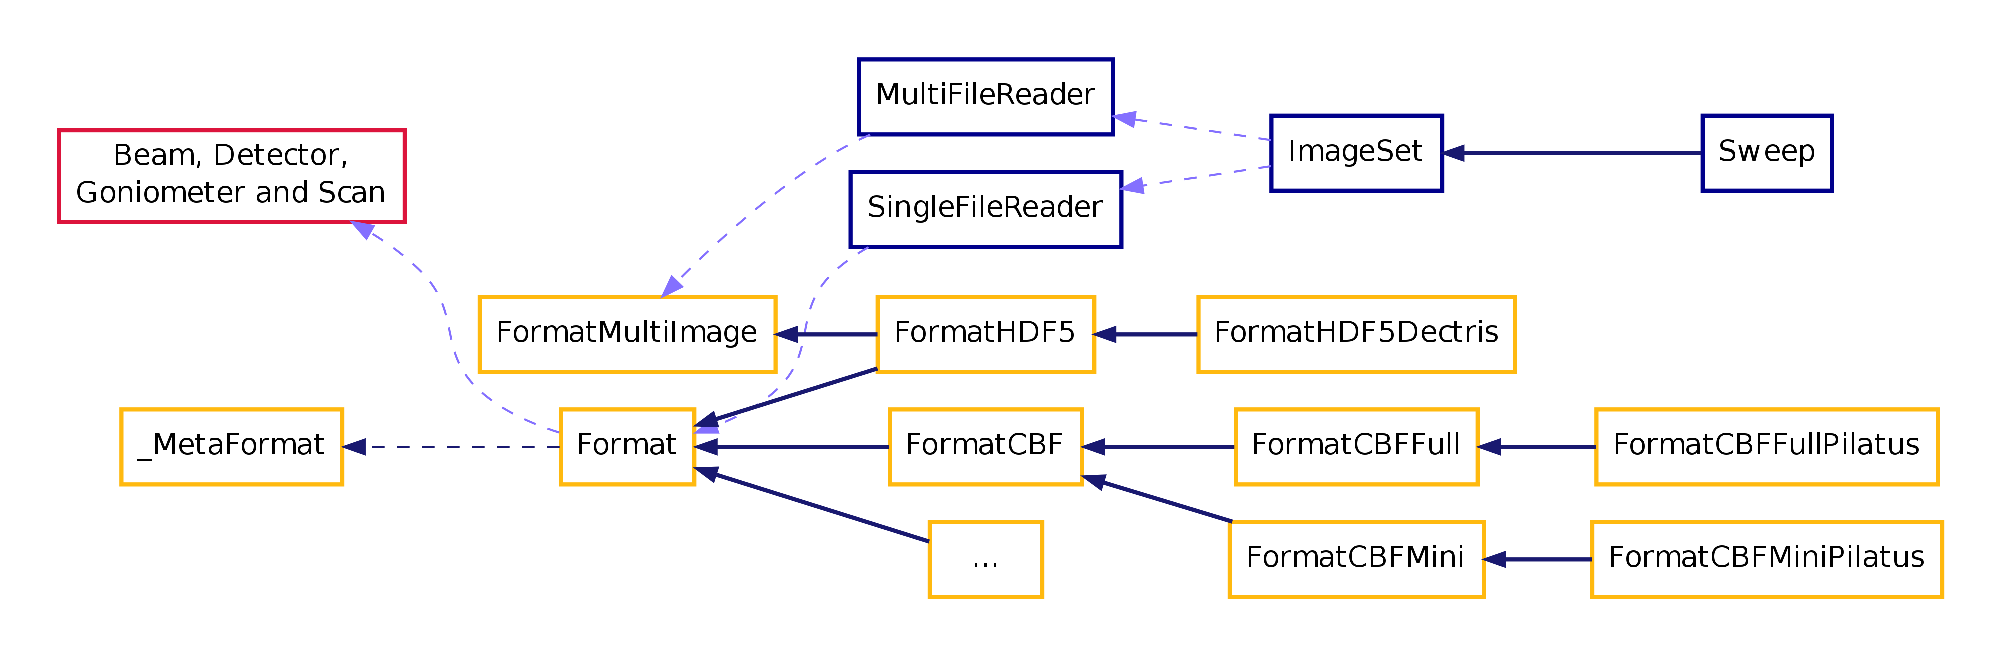
\includegraphics[width=\columnwidth]{./Figures/fig1.eps}
\end{figure}
\twocolumn

\onecolumn
\begin{figure}
\label{figure: geometry}
\centering
\caption{The description of diffraction geometry for the rotation method using 
dxtbx models [FIXME: need larger fonts]. A monochromatic X-ray beam is 
represented by the wavevector \(\bm{s_0}\), which intersects a sample rotation 
axis, given by the unit vector \(\bm{e}\), at the origin of the reciprocal 
laboratory coordinate system. An abstract detector plane \(\bm{k}\) is described 
in the aligned real space laboratory coordinate system with an origin vector 
\(\bm{d^k_0}\) and a pair of orthogonal basis vectors 
\((\bm{d^k_x}, \bm{d^k_y})\) with units of millimetres. The detector model 
provides a pair of limits, \(lim_x\) and \(lim_y\), forming a bounded rectangular 
panel within the plane. A crystal model complements the dxtbx geometry models, 
with its setting expressed in a \(\phi-axis\) frame (aligned to the reciprocal 
laboratory frame at a rotation angle of \(\phi = 0^{\circ}\)) by the matrix 
\(\bm{UB}\). Diffraction is represented by the wavevector \(\bm{s}\), which may 
be scaled to the point X, Y at which it meets the detector panel, in the panel's 
attached coordinate frame.}
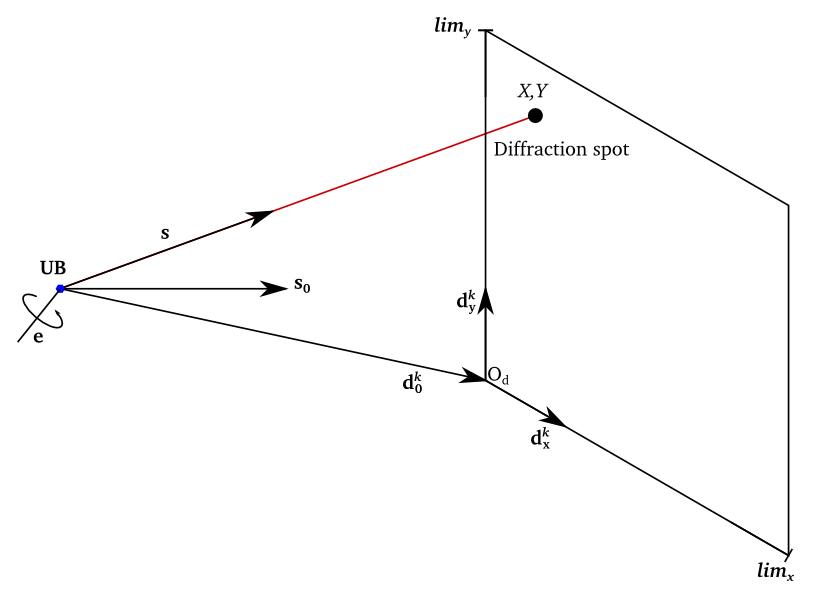
\includegraphics[width=\textwidth]{./Figures/fig2.eps}
\end{figure}
\twocolumn

\end{document}
